%%%%%%%%%%%%%%%%%%%%%%%%%%%%%%%%%%%%%%%%%
% Programming/Coding Assignment
% LaTeX Template
%
% This template has been downloaded from:
% http://www.latextemplates.com
%
% Original author:
% Ted Pavlic (http://www.tedpavlic.com)
%
% Note:
% The \lipsum[#] commands throughout this template generate dummy text
% to fill the template out. These commands should all be removed when 
% writing assignment content.
%
% This template uses a Perl script as an example snippet of code, most other
% languages are also usable. Configure them in the "CODE INCLUSION 
% CONFIGURATION" section.
%
%%%%%%%%%%%%%%%%%%%%%%%%%%%%%%%%%%%%%%%%%

%----------------------------------------------------------------------------------------
%	PACKAGES AND OTHER DOCUMENT CONFIGURATIONS
%----------------------------------------------------------------------------------------

\documentclass{article}

\usepackage{fancyhdr} % Required for custom headers
\usepackage{lastpage} % Required to determine the last page for the footer
\usepackage{extramarks} % Required for headers and footers
\usepackage[usenames,dvipsnames]{color} % Required for custom colors
\usepackage{graphicx} % Required to insert images
\usepackage{listings} % Required for insertion of code
\usepackage{courier} % Required for the courier font
\usepackage{lipsum} % Used for inserting dummy 'Lorem ipsum' text into the template
\usepackage{setspace}
\usepackage{color}
\usepackage{comment}
\usepackage{caption}

\usepackage{hyperref}
\usepackage{natbib}
\usepackage{underscore}
\usepackage{subfigure}


\hypersetup{
    colorlinks=true,
    linkcolor=blue,
    filecolor=magenta,      
    urlcolor=cyan,
    breaklinks=true
}

%\usepackage[]{algorithm2e}
\usepackage{pdfpages}




%For python inclusion (http://widerin.org/blog/syntax-highlighting-for-python-scripts-in-latex-documents)
\definecolor{Code}{rgb}{0,0,0}
\definecolor{Decorators}{rgb}{0.5,0.5,0.5}
\definecolor{Numbers}{rgb}{0.5,0,0}
\definecolor{MatchingBrackets}{rgb}{0.25,0.5,0.5}
\definecolor{Keywords}{rgb}{0,0,1}
\definecolor{self}{rgb}{0,0,0}
\definecolor{Strings}{rgb}{0,0.63,0}
\definecolor{Comments}{rgb}{0,0.63,1}
\definecolor{Backquotes}{rgb}{0,0,0}
\definecolor{Classname}{rgb}{0,0,0}
\definecolor{FunctionName}{rgb}{0,0,0}
\definecolor{Operators}{rgb}{0,0,0}
\definecolor{Background}{rgb}{0.98,0.98,0.98}

% Margins
\topmargin=-0.45in
\evensidemargin=0in
\oddsidemargin=0in
\textwidth=6.5in
\textheight=9.0in
\headsep=0.25in

\linespread{1.1} % Line spacing

% Set up the header and footer
\pagestyle{fancy}
\lhead{\hmwkAuthorName} % Top left header
%\chead{\hmwkClass\ (\hmwkClassInstructor\ \hmwkClassTime): \hmwkTitle} % Top center head
\chead{\hmwkClass\ (\hmwkClassInstructor): \hmwkTitle} % Top center head
\rhead{\firstxmark} % Top right header
\lfoot{\lastxmark} % Bottom left footer
\cfoot{} % Bottom center footer
\rfoot{Page\ \thepage\ of\ \protect\pageref{LastPage}} % Bottom right footer
\renewcommand\headrulewidth{0.4pt} % Size of the header rule
\renewcommand\footrulewidth{0.4pt} % Size of the footer rule

\setlength\parindent{0pt} % Removes all indentation from paragraphs

%----------------------------------------------------------------------------------------
%	CODE INCLUSION CONFIGURATION
%----------------------------------------------------------------------------------------

\definecolor{MyDarkGreen}{rgb}{0.0,0.4,0.0} % This is the color used for comments
\lstloadlanguages{Perl} % Load Perl syntax for listings, for a list of other languages supported see: ftp://ftp.tex.ac.uk/tex-archive/macros/latex/contrib/listings/listings.pdf
\lstset{language=Perl, % Use Perl in this example
        frame=single, % Single frame around code
        basicstyle=\small\ttfamily, % Use small true type font
        keywordstyle=[1]\color{Blue}\bf, % Perl functions bold and blue
        keywordstyle=[2]\color{Purple}, % Perl function arguments purple
        keywordstyle=[3]\color{Blue}\underbar, % Custom functions underlined and blue
        identifierstyle=, % Nothing special about identifiers                                         
        commentstyle=\usefont{T1}{pcr}{m}{sl}\color{MyDarkGreen}\small, % Comments small dark green courier font
        stringstyle=\color{Purple}, % Strings are purple
        showstringspaces=false, % Don't put marks in string spaces
        tabsize=5, % 5 spaces per tab
        %
        % Put standard Perl functions not included in the default language here
        morekeywords={rand},
        %
        % Put Perl function parameters here
        morekeywords=[2]{on, off, interp},
        %
        % Put user defined functions here
        morekeywords=[3]{test},
       	%
        morecomment=[l][\color{Blue}]{...}, % Line continuation (...) like blue comment
        numbers=left, % Line numbers on left
        firstnumber=1, % Line numbers start with line 1
        numberstyle=\tiny\color{Blue}, % Line numbers are blue and small
        stepnumber=5 % Line numbers go in steps of 5
}

% Creates a new command to include a perl script, the first parameter is the filename of the script (without .pl), the second parameter is the caption
\newcommand{\perlscript}[2]{
\begin{itemize}
\item[]\lstinputlisting[caption=#2,label=#1]{#1.pl}
\end{itemize}
}


%----------------------------------------------------------------------------------------
%	DOCUMENT STRUCTURE COMMANDS
%	Skip this unless you know what you're doing
%----------------------------------------------------------------------------------------

% Header and footer for when a page split occurs within a problem environment
\newcommand{\enterProblemHeader}[1]{
\nobreak\extramarks{#1}{#1 continued on next page\ldots}\nobreak
\nobreak\extramarks{#1 (continued)}{#1 continued on next page\ldots}\nobreak
}

% Header and footer for when a page split occurs between problem environments
\newcommand{\exitProblemHeader}[1]{
\nobreak\extramarks{#1 (continued)}{#1 continued on next page\ldots}\nobreak
\nobreak\extramarks{#1}{}\nobreak
}

\setcounter{secnumdepth}{0} % Removes default section numbers
\newcounter{homeworkProblemCounter} % Creates a counter to keep track of the number of problems

\newcommand{\homeworkProblemName}{}
\newenvironment{homeworkProblem}[1][Problem \arabic{homeworkProblemCounter}]{ % Makes a new environment called homeworkProblem which takes 1 argument (custom name) but the default is "Problem #"
\stepcounter{homeworkProblemCounter} % Increase counter for number of problems
\renewcommand{\homeworkProblemName}{#1} % Assign \homeworkProblemName the name of the problem
\section{\homeworkProblemName} % Make a section in the document with the custom problem count
\enterProblemHeader{\homeworkProblemName} % Header and footer within the environment
}{
\exitProblemHeader{\homeworkProblemName} % Header and footer after the environment
}

\newcommand{\problemAnswer}[1]{ % Defines the problem answer command with the content as the only argument
\noindent\framebox[\columnwidth][c]{\begin{minipage}{0.98\columnwidth}#1\end{minipage}} % Makes the box around the problem answer and puts the content inside
}

\newcommand{\homeworkSectionName}{}
\newenvironment{homeworkSection}[1]{ % New environment for sections within homework problems, takes 1 argument - the name of the section
\renewcommand{\homeworkSectionName}{#1} % Assign \homeworkSectionName to the name of the section from the environment argument
\subsection{\homeworkSectionName} % Make a subsection with the custom name of the subsection
\enterProblemHeader{\homeworkProblemName\ [\homeworkSectionName]} % Header and footer within the environment
}{
\enterProblemHeader{\homeworkProblemName} % Header and footer after the environment
}

%----------------------------------------------------------------------------------------
%	NAME AND CLASS SECTION
%----------------------------------------------------------------------------------------

\newcommand{\hmwkTitle}{Assignment\ \#10 } % Assignment title
%\newcommand{\hmwkDueDate}{Monday,\ January\ 1,\ 2012} % Due date
\newcommand{\hmwkClass}{Introduction to Web Science} % Course/class
%\newcommand{\hmwkClassTime}{10:30am} % Class/lecture time
\newcommand{\hmwkClassInstructor}{Dr. Nelson} % Teacher/lecturer
\newcommand{\hmwkAuthorName}{Alexander Nwala} % Your name

%----------------------------------------------------------------------------------------
%	TITLE PAGE
%----------------------------------------------------------------------------------------

\title{
\vspace{2in}
\textmd{\textbf{\hmwkClass:\ \hmwkTitle}}\\
%\normalsize\vspace{0.1in}\small{Due\ on\ \hmwkDueDate}\\
%\vspace{0.1in}\large{\textit{\hmwkClassInstructor\ \hmwkClassTime}}
\vspace{0.1in}\large{\textit{\hmwkClassInstructor}}
\vspace{3in}
}

\author{\textbf{\hmwkAuthorName}}
\date{Thursday, December 11, 2014} % Insert date here if you want it to appear below your name

%----------------------------------------------------------------------------------------

\begin{document}

\maketitle



%----------------------------------------------------------------------------------------
%	TABLE OF CONTENTS
%----------------------------------------------------------------------------------------

%\setcounter{tocdepth}{1} % Uncomment this line if you don't want subsections listed in the ToC

\newpage
\tableofcontents
\newpage

%----------------------------------------------------------------------------------------
%	PROBLEM 1
%----------------------------------------------------------------------------------------

% To have just one problem per page, simply put a \clearpage after each problem

\begin{homeworkProblem}

Choose a blog or a newsfeed (or something similar as long as it has
an Atom or RSS feed).  It should be on a topic or topics of which you
are qualified to provide classification training data.  In other words,
choose something that you enjoy and are knowledgable of.  Find a feed
with at least 100 entries.\\

Create between four and eight different categories for the entries
in the feed:\\

examples: 

\begin{verbatim}
    - work, class, family, news, deals
    - liberal, conservative, moderate, libertarian
    - sports, local, financial, national, international, entertainment
    - metal, electronic, ambient, folk, hip-hop, pop
\end{verbatim}

Download and process the pages of the feed as per the week 12 
class slides. 

%\problemAnswer
%{
    \begin{verbatim}\end{verbatim}
    \textbf{SOLUTION 1}\\

    The solution for this problem is outlined by the following steps:
    \begin{enumerate}

    \item \textbf{Select a blog:} My goal was to select a blog with entries over 100 (from Blogspot) with as much heterogenous content as possible. Given this criteria, I selected \url{http://stevegilliard.blogspot.com/}

    \item \textbf{Extract entries from blog:} The Atom feed of the blog was extracted and saved into an XML file due to Listing 1. 300 entries were collected in order to have enough data in the event of errors.

    \lstinputlisting[breaklines=true, caption=Save Blog Entries to XML file]{getXMLEntriesSnippet.py}

    \item \textbf{Manually classify all entries:} After inspecting the blog entries, I chose 4 classes:

    \begin{verbatim}
    Politics - For Politics related entries
    Story - For News and narratives on different topics
    Law - For Crime and Law enforcement related entries
    Misc - For topics which clearly do not belong to the previous classes
    \end{verbatim}

    \item \textbf{Partition data into 2 sets:} The 100 entries from the blog were split into 2 partitions (first 50 and last 50 entries). Table 1. is a summary of the class distribution for the 100 blog entries of the 2 sets.

    \begin{verbatim}
        The file 50nBlogTrainingDataSource.txt contains the first set of:
            <BlogEntryTitle, BlogEntrySummary, UserAssignedClassLabel>
        The file 50nBlogTestDataSource.txt contains the second set of:
            <BlogEntryTitle, BlogEntrySummary, UserAssignedClassLabel>
    \end{verbatim}

    \end{enumerate}
    \begin{table}
        \caption{Distribution of Classes} % title of Table
        \centering % used for centering table
        \begin{tabular}{c | c | c | c } % centered columns (4 columns)
        \hline\hline %inserts double horizontal lines
        ITEM & Class & First 50 & Second 50 \\ [0.5ex] % inserts table 
        %heading
        \hline \hline% inserts single horizontal line
        1   &   Politics    &   26  & 13\\ \hline
        2   &   Story    &   15 & 22\\ \hline
        3   &   Law    &   3 & 6\\ \hline
        4 & Misc & 6 & 9\\ [1ex] 
        \hline %inserts single line
        \end{tabular}
        \label{table:nonlin} % is used to refer this table in the text
    \end{table}
    %\begin{figure}
    %    \caption{Distribution of Pages}
    %    \subfigure{\includegraphics[width=\textwidth]{../Rplots.pdf}}
    %\end{figure}

%}



\end{homeworkProblem}

%----------------------------------------------------------------------------------------
%	PROBLEM 2
%----------------------------------------------------------------------------------------
\begin{homeworkProblem}

Manually classify the first 50 entries, and then classify (using
the fisher classifier) the remaining 50 entries. Report the cprob()
values for the 50 titles as well.  From the title or entry itself,
specify the 1-, 2-, or 3-gram that you used for the string to
classify.  Do not repeat strings; you will have 50 unique strings.
For example, in these titles the string used is marked with *s:\\

*Rachel Goswell* - ``Waves Are Universal'' (LP Review)\\
The *Naked and Famous* - ``Passive Me, Aggressive You'' (LP Review)\\
*Negativland* - ``Live at Lewis's, Norfolk VA, November 21, 1992'' (concert)\\
Negativland - ``*U2*'' (LP Review)\\

Note how ``Negativland'' is not repeated as a classification string.\\

Create a table with the title, the string used for classification,
cprob(), predicted category, and actual category.

\begin{verbatim}\end{verbatim}
\textbf{SOLUTION 2}\\


The solution for this problem is outlined by the following steps:
\begin{enumerate}

\item \textbf{Train model:} Listing 2. (myFisherModelInTrainingAndTesting) utilizes a modified version of the PCI book's \cite{pciBook} feedfilter.py read method (nonInteractiveRead). The modification facilitates automated testing and training (not user-interactive) by operating on an input file which contains the user supplied class labels.\\

Given that the same function is used for training and testing, a call to myFisherModelInTrainingAndTesting is made supplying the ``train'' argument. The result of the training is written into a database file (stevegilliard.db)

\lstinputlisting[breaklines=true, caption=Fisher Model]{fisherModelSnippet.py}

\item \textbf{Test model:} Utilizing the model learned during training, the same function (myFisherModelInTrainingAndTesting) was called to test the model by supplying the ``test'' argument. Table 2. summarizes the result of the test. The string used for testing was the blog contents (summaries) and is omitted from the table due to its length. Also Table 3. shows the first 50 entries used to train the model. Table 2. is three entries short due to absent weighted probability values associated with three entries.


\begin{table}
    \caption{Fisher Method Test Result For getword Function} % title of Table
    \centering % used for centering table\begin{tabular}{m{5cm} c}
    \begin{tabular}{c | c | c | c | c } % centered columns (4 columns)
    \hline\hline %inserts double horizontal lines
    
    ITEM & ENTRY-TITLE & CPROB & PRED-LABEL & ACTUAL-LABEL \\ [0.5ex] % inserts table 
    %heading
    \hline \hline% inserts single horizontal line

    1   &   Mr. Sulu Phasers Tim Hardaway    &  0.2500  &  story &  story\\ \hline
    2   &   Too close for comfort       &  0.3693  &  politics &  politics\\ \hline
    3   &   Middle School?         &  0.2500  &  politics &  politics\\ \hline
    4   &   No kids for gays    &  0.3147  &  politics &  politics\\ \hline
    5   &   HDTV       &  0.3693  &  story &  story\\ \hline
    6   &   Change sometimes isn't so fast         &  0.2500  &  story &  story\\ \hline
    7   &   More idiocy    &  0.2500  &  politics &  politics\\ \hline
    8   &   Yawn, Hillary's In       &  0.2685  &  politics &  politics\\ \hline
    9   &   Scumbags in action         &  0.2500  &  politics &  politics\\ \hline
    10   &  The battle of the exploding pigs    &  0.3693  &  politics &  politics\\ \hline

    11   &   Racial Row on UK show            &  0.3693  &  politics &  story\\ \hline
    12   &   No spanking    &  0.3147  &  politics &  story\\ \hline
    13   &   Provoking Sadr      &  0.6018  &  politics &  politics\\ \hline
    14   &   Jenna writes a book            &  0.2500  &  story &  misc\\ \hline
    15   &   Only in Washington    &  0.5058  &  politics &  politics\\ \hline
    16   &   Oooops      &  0.2500  &  politics &  story\\ \hline
    17   &   Another 9/11 tragedy            &  0.3693  &  story &  story\\ \hline
    18   &   Time to serve    &  0.2500  &  politics &  misc\\ \hline
    19   &   About going to Walter Reed      &  0.3693  &  story &  story\\ \hline

    20   &   Voir Dire from hell            &  0.8965  &  politics & law\\ \hline 
    21   &   Simple point    &  0.3693  &  misc & misc\\ \hline
    22   &   Fading away      &  0.8227  &  politics & politics\\ \hline
    23   &   We're playing you            &  0.8333  &  politics & story\\ \hline
    24   &   Libby on trial    &  0.3147  &  politics & law\\ \hline
    25   &   The Car Wreck of American TV      &  0.3693  &  politics & misc\\ \hline
    26   &   No more actors            &  0.2500  &  story & story\\ \hline
    27   &   Good luck, Jane    &  0.2689  &  politics & misc\\ \hline
    28   &   More dead in Iraq      &  0.6132  &  politics & law\\ \hline
    29   &   The good old days my ass            &  0.1575  &  politics & politics\\ \hline

    30   &   A simple question    &  0.2500  &  politics &  politics\\ \hline
    31   &   What bubble?      &  0.3147  &  politics &  story\\ \hline
    32   &   Idiocy in action            &  0.2500  &  story &  story\\ \hline
    33   &   Yeah, attacking the Mahdi Army will happen    &  0.5855  &  politics &  politics\\ \hline
    34   &   What can I do?      &  0.5855  &  politics &  story\\ \hline
    35   &   Marine murdered for insurance?            &  0.8965  &  story &  law\\ \hline
    36   &   Hey, it just happened    &  0.3147  &  politics &  story\\ \hline
    37   &   Why the fuck is he making military policy      &  0.2500  &  politics &  politics\\ \hline
    38   &   You have to be kidding            &  0.2500  &  politics &  story\\ \hline
    39   &   Bush will lose the country    &  0.3693  &  politics &  politics\\ \hline

    40   &   Pointless      &  0.2500  &  politics &  story\\ \hline
    41   &   Better to  drop FAE's instead            &  0.2500  &  politics &  story\\ \hline
    42   &   How stupid can you be    &  0.2500  &  story &  story\\ \hline
    43   &   Madness in action      &  0.3147  &  politics &  politics\\ \hline
    44   &   They don't want us            &  0.2500  &  politics &  politics\\ \hline
    45   &   Sucker    &  0.2500  &  politics &  story\\ \hline
    46   &   Silicone    &  0.3693  &  politics &  misc\\ \hline

    47  &  Idiocy in action        &  0.2012  &  politics & story\\ [1ex] 
    \hline %inserts single line
    \end{tabular}
    \label{table:nonlin} % is used to refer this table in the text
\end{table}

\begin{table}
    \caption{Fisher Method Training Dataset} % title of Table
    \centering % used for centering table\begin{tabular}{m{5cm} c}
    \begin{tabular}{c | c | c } % centered columns (4 columns)
    \hline\hline %inserts double horizontal lines
    
    ITEM & ENTRY-TITLE & ACTUAL-LABEL \\ [0.5ex] % inserts table 
    %heading
    \hline \hline% inserts single horizontal line

    1   &   I told you this would happen    &   politics\\ \hline
    2   &   He  has affliliations   &   politics\\ \hline
    3   &   Reality Check   &   politics\\ \hline
    4   &   Bush's plan falling apart   &   politics\\ \hline
    5   &   A history lesson    &   politics\\ \hline
    6   &   This makes me laugh &   misc\\ \hline
    7   &   Talk or no talk &   misc\\ \hline
    8   &   A nervous WH    &   politics\\ \hline
    9   &   www.thenewsblog.net &   misc\\ \hline
    10  &   Thank you, Jesus    &   story\\ \hline
    11  &   Shut yer festerin' gob  &   politics\\ \hline
    12  &   Give me back my airmen  &   politics\\ \hline
    13  &   Max responds    &   politics\\ \hline
    14  &   Here we go again    &   law\\ \hline
    15  &   Favorite Egg recipe &   misc\\ \hline
    16  &   WH lies &   politics\\ \hline
    17  &   I don't know    &   story\\ \hline
    18  &   She wanted unemployment?    &   story\\ \hline
    19  &   Racist pig speaks   &   story\\ \hline
    20  &   Bush's fantasyland  &   politics\\ \hline
    21  &   Weird weather cures &   story\\ \hline
    22  &   Idiot   &   story\\ \hline
    23  &   Are you kidding?    &   politics\\ \hline
    24  &   Bwaaaah &   politics\\ \hline
    25  &   The war was wrong   &   politics\\ \hline
    26  &   Fucking Moron   &   politics\\ \hline
    27  &   When the law doesn't work, try blackmail    &   politics\\ \hline
    28  &   We oppose the war   &   politics\\ \hline
    29  &   Black life means nothing  to Lieberman  &   politics\\ \hline
    30  &   The Hamilton Rule   &   politics\\ \hline
    31  &   Where is Hillary?   &   politics\\ \hline
    32  &   So who did this?    &   politics\\ \hline
    33  &   Dear Max    &   misc\\ \hline
    34  &   Nothing like Vietnam    &   story\\ \hline
    35  &   A real GI Bill  &   politics\\ \hline
    36  &   Jesus   &   story\\ \hline
    37  &   Be greatful, Iraqis &   politics\\ \hline
    38  &   This isn't in the plans for the Kurds   &   politics\\ \hline
    39  &   Duh &   story\\ \hline
    40  &   Beckham in America  &   misc\\ \hline
    41  &   What are people afraid of?  &   story\\ \hline
    42  &   Gunpoint at Democracy   &   law\\ \hline
    43  &   No kidding  &   politics\\ \hline
    44  &   You bet your life   &   story\\ \hline
    45  &   Leave Iran Alone    &   story\\ \hline
    46  &   Failure &   story\\ \hline
    47  &   Spocko v Disney &   story\\ \hline
    48  &   Yes, you need to apologize, you goddamn redneck bastard &   story\\ \hline
    49  &   Mercenary murder in Iraq?   &   law\\ \hline

    50  &   Attacking Iran  &   politics\\ [1ex] 
    \hline %inserts single line
    \end{tabular}
    \label{table:nonlin} % is used to refer this table in the text
\end{table}

\end{enumerate}

\end{homeworkProblem}

%----------------------------------------------------------------------------------------
%   PROBLEM 3
%----------------------------------------------------------------------------------------
\begin{homeworkProblem}

Assess the performance of your classifier in each of your categories
by computing precision, recall, and F1.  Note that the definitions
of precisions and recall are slightly different in the context of
classification; see:

\url{http://en.wikipedia.org/wiki/Precision_and_recall#Definition_.28classification_context.29}

and

\url{http://en.wikipedia.org/wiki/F1_score}

\begin{verbatim}\end{verbatim}
\textbf{SOLUTION 3}\\


The solution for this problem is outlined by the following steps:
\begin{enumerate}

\item \textbf{Generate confusion matrix and calculate precision/recall/F1 measures:} This was achieved due to Listing 3. which utilized the scikit-learn
Machine Learning in Python library \cite{sklearn}

\lstinputlisting[breaklines=true, caption=Calculate Precision]{calculatePrecisionSnippet.py}

Figure 1. outlines the confusion matrix due to Listing 3.
%As seen from Figure 1. the model produces the highest True Positive values in the Politics and Story class - this is not surprising due to the large amount of the samples belonging to these classes. The reverse applies to the Law and Misc classes. \\

The following represent the numeric values corresponding to the confusion matrix. Table 4. outlines the precision of the various classes.
The sum of true positives and false positives are equal to zero for some labels such as Law, this is reason why the precision/recall/F1 is ill defined for the Law class.

\begin{verbatim}
               p   s  l  m
            p [12  0  0  0]
            s [15  5  0  0]
            l [ 4  2  0  0]
            m [ 5  3  0  1]

            p = Politics, s = Story, l = Law, m = Misc
\end{verbatim}

\begin{table}
        \caption{Precision/Recall/F1 Measures 50/50 Split With getword Function} % title of Table
        \centering % used for centering table
        \begin{tabular}{c | c | c | c | c } % centered columns (4 columns)
        \hline\hline %inserts double horizontal lines
        ITEM & Class & Precision & Recall & F1 \\ [0.5ex] % inserts table 
        %heading
        \hline \hline% inserts single horizontal line
        1   &   Politics    &   0.3333  & 1.0000 & 0.5000\\ \hline
        2   &   Story    &   0.5000 & 0.2500 & 0.3333\\ \hline
        3   &   Law    &   0.0000 & 0.0000 & 0.0000 \\ \hline
        4 & Misc & 1.0000 & 0.1111 & 0.2000\\ [1ex] 
        \hline %inserts single line
        \end{tabular}
        \label{table:nonlin} % is used to refer this table in the text
\end{table}

\begin{figure}[h]
    \caption{Confusion Matrix For 50/50 Split}
    %\subfigure{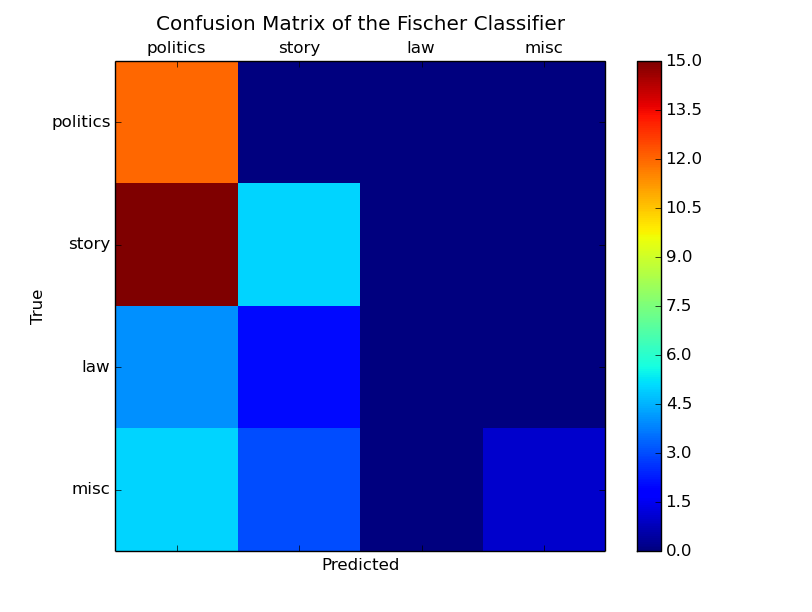
\includegraphics[width=\textwidth,height=\textheight]{confusionMatrix.png}}
    \subfigure{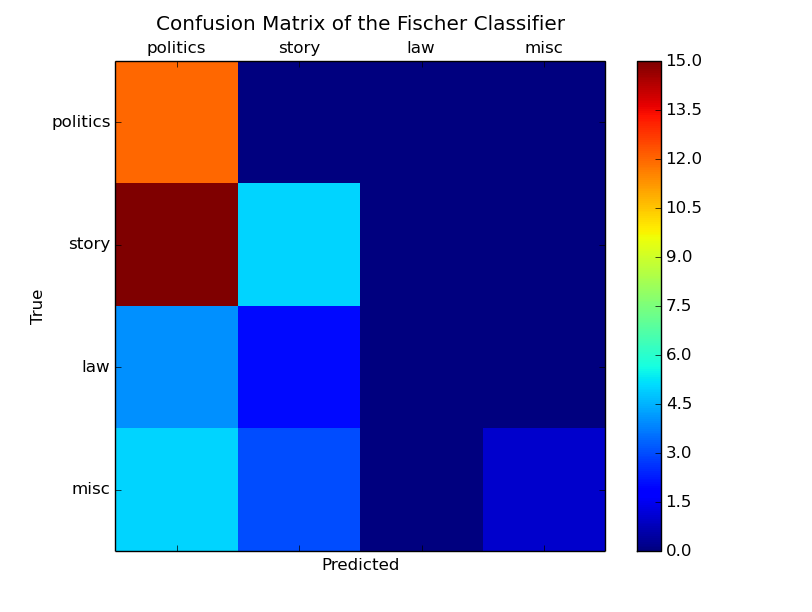
\includegraphics[width=\textwidth]{confusionMatrix.png}}
\end{figure}


\end{enumerate}

\end{homeworkProblem}


%----------------------------------------------------------------------------------------
%   PROBLEM 4
%----------------------------------------------------------------------------------------
\begin{homeworkProblem}

Redo questions 2 \& 3, but with manually train 90 entries and 
then classify the remaining 10.\\

Then redo questions 2 \& 3, but with the extensions on slide 26
and pp. 136--138.  Fully discuss the changes you've made.\\

Which method (more training vs. better features) gave better improvement
over your baseline?  Why do you think that is?\\

\begin{verbatim}\end{verbatim}
\textbf{SOLUTION 4}\\


The solution for this problem is outlined by the following steps:
\begin{enumerate}

\item \textbf{Train and test with 90/10 split:} This was achieved in the same manner as the 50/50 case (50 training dataset, 50 dataset), but this time with 90 entries for training and 10 entries for test. In addition, Table 5. outlines the precision/recall/F1 scores for each blog entry while Table 6. outlines the cprob/predition/actual label for each entry. And below is the confusion matrix.

\begin{verbatim}
               p s l m
            p [1 0 0 0]
            s [3 1 0 0]
            l [0 0 0 0]
            m [2 2 0 1]

            p = Politics, s = Story, l = Law, m = Misc
\end{verbatim}

\begin{table}
        \caption{Precision/Recall/F1 Measures For 90/10 Split} % title of Table
        \centering % used for centering table
        \begin{tabular}{c | c | c | c | c } % centered columns (4 columns)
        \hline\hline %inserts double horizontal lines
        ITEM & Class & Precision & Recall & F1 \\ [0.5ex] % inserts table 
        %heading
        \hline \hline% inserts single horizontal line
        1   &   Politics    &   0.1667  & 1.0000 & 0.2857\\ \hline
        2   &   Story    &   0.3333 & 0.2500 & 0.2857\\ \hline
        3   &   Law    &   0.0000 & 0.0000 & 0.0000 \\ \hline
        4 & Misc & 1.0000 & 0.1111 & 0.3333\\ [1ex] 
        \hline %inserts single line
        \end{tabular}
        \label{table:nonlin} % is used to refer this table in the text
\end{table}

\begin{table}
    \caption{Fisher Method Test Result For 90/10 Split}  % title of Table
    \centering % used for centering table\begin{tabular}{m{5cm} c}
    \begin{tabular}{c | c | c | c | c} % centered columns (4 columns)
    \hline\hline %inserts double horizontal lines
    
    ITEM & ENTRY-TITLE & CPROB & PRED-LABEL & ACTUAL-LABEL \\ [0.5ex] % inserts table 
    %heading
    \hline \hline% inserts single horizontal line

    1   &   Mr. Sulu Phasers Tim Hardaway    &   0.2500 & story & misc\\ \hline
    2   &   Despite total ignorance, I support this idea   &   0.2695 & politics & story\\ \hline
    3   &   Time to serve   &   0.2500 & politics & misc\\ \hline
    4   &   Simple point   &   0.1062 & misc & misc\\ \hline
    5   &   We're playing you    &   0.4857 & story & story\\ \hline
    6   &   Good luck, Jane &   0.2659 & politics & misc\\ \hline
    7   &   A simple question &   0.2500 & politics & politics\\ \hline
    8   &   Pointless    &   0.3345 & politics & story\\ \hline
    9   &   Sucker &   0.2500 & politics & story\\ \hline

    10  &   Silicone  &   0.1945 & story & misc\\ [1ex] 
    \hline %inserts single line
    \end{tabular}
    \label{table:nonlin} % is used to refer this table in the text
\end{table}

\begin{figure}[h]
    \caption{Confusion Matrix For 90/10 Split}
    %\subfigure{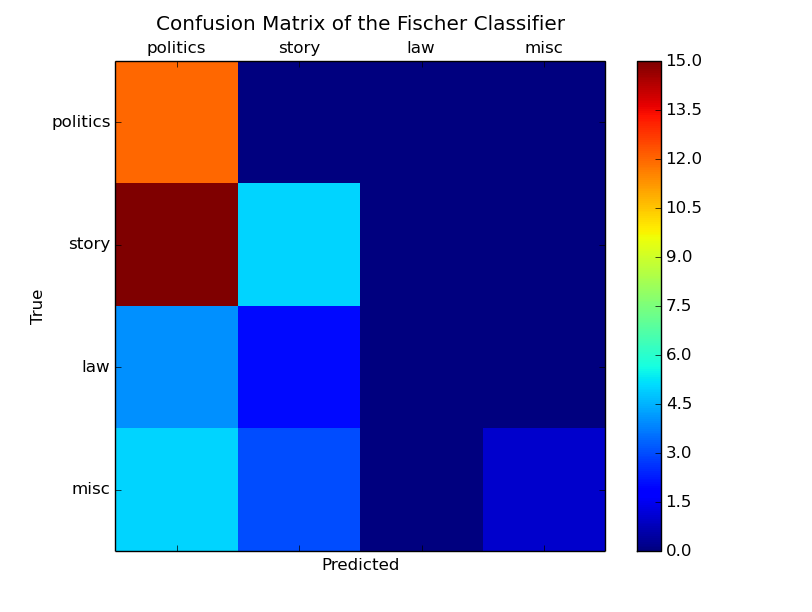
\includegraphics[width=\textwidth,height=\textheight]{confusionMatrix.png}}
    \subfigure{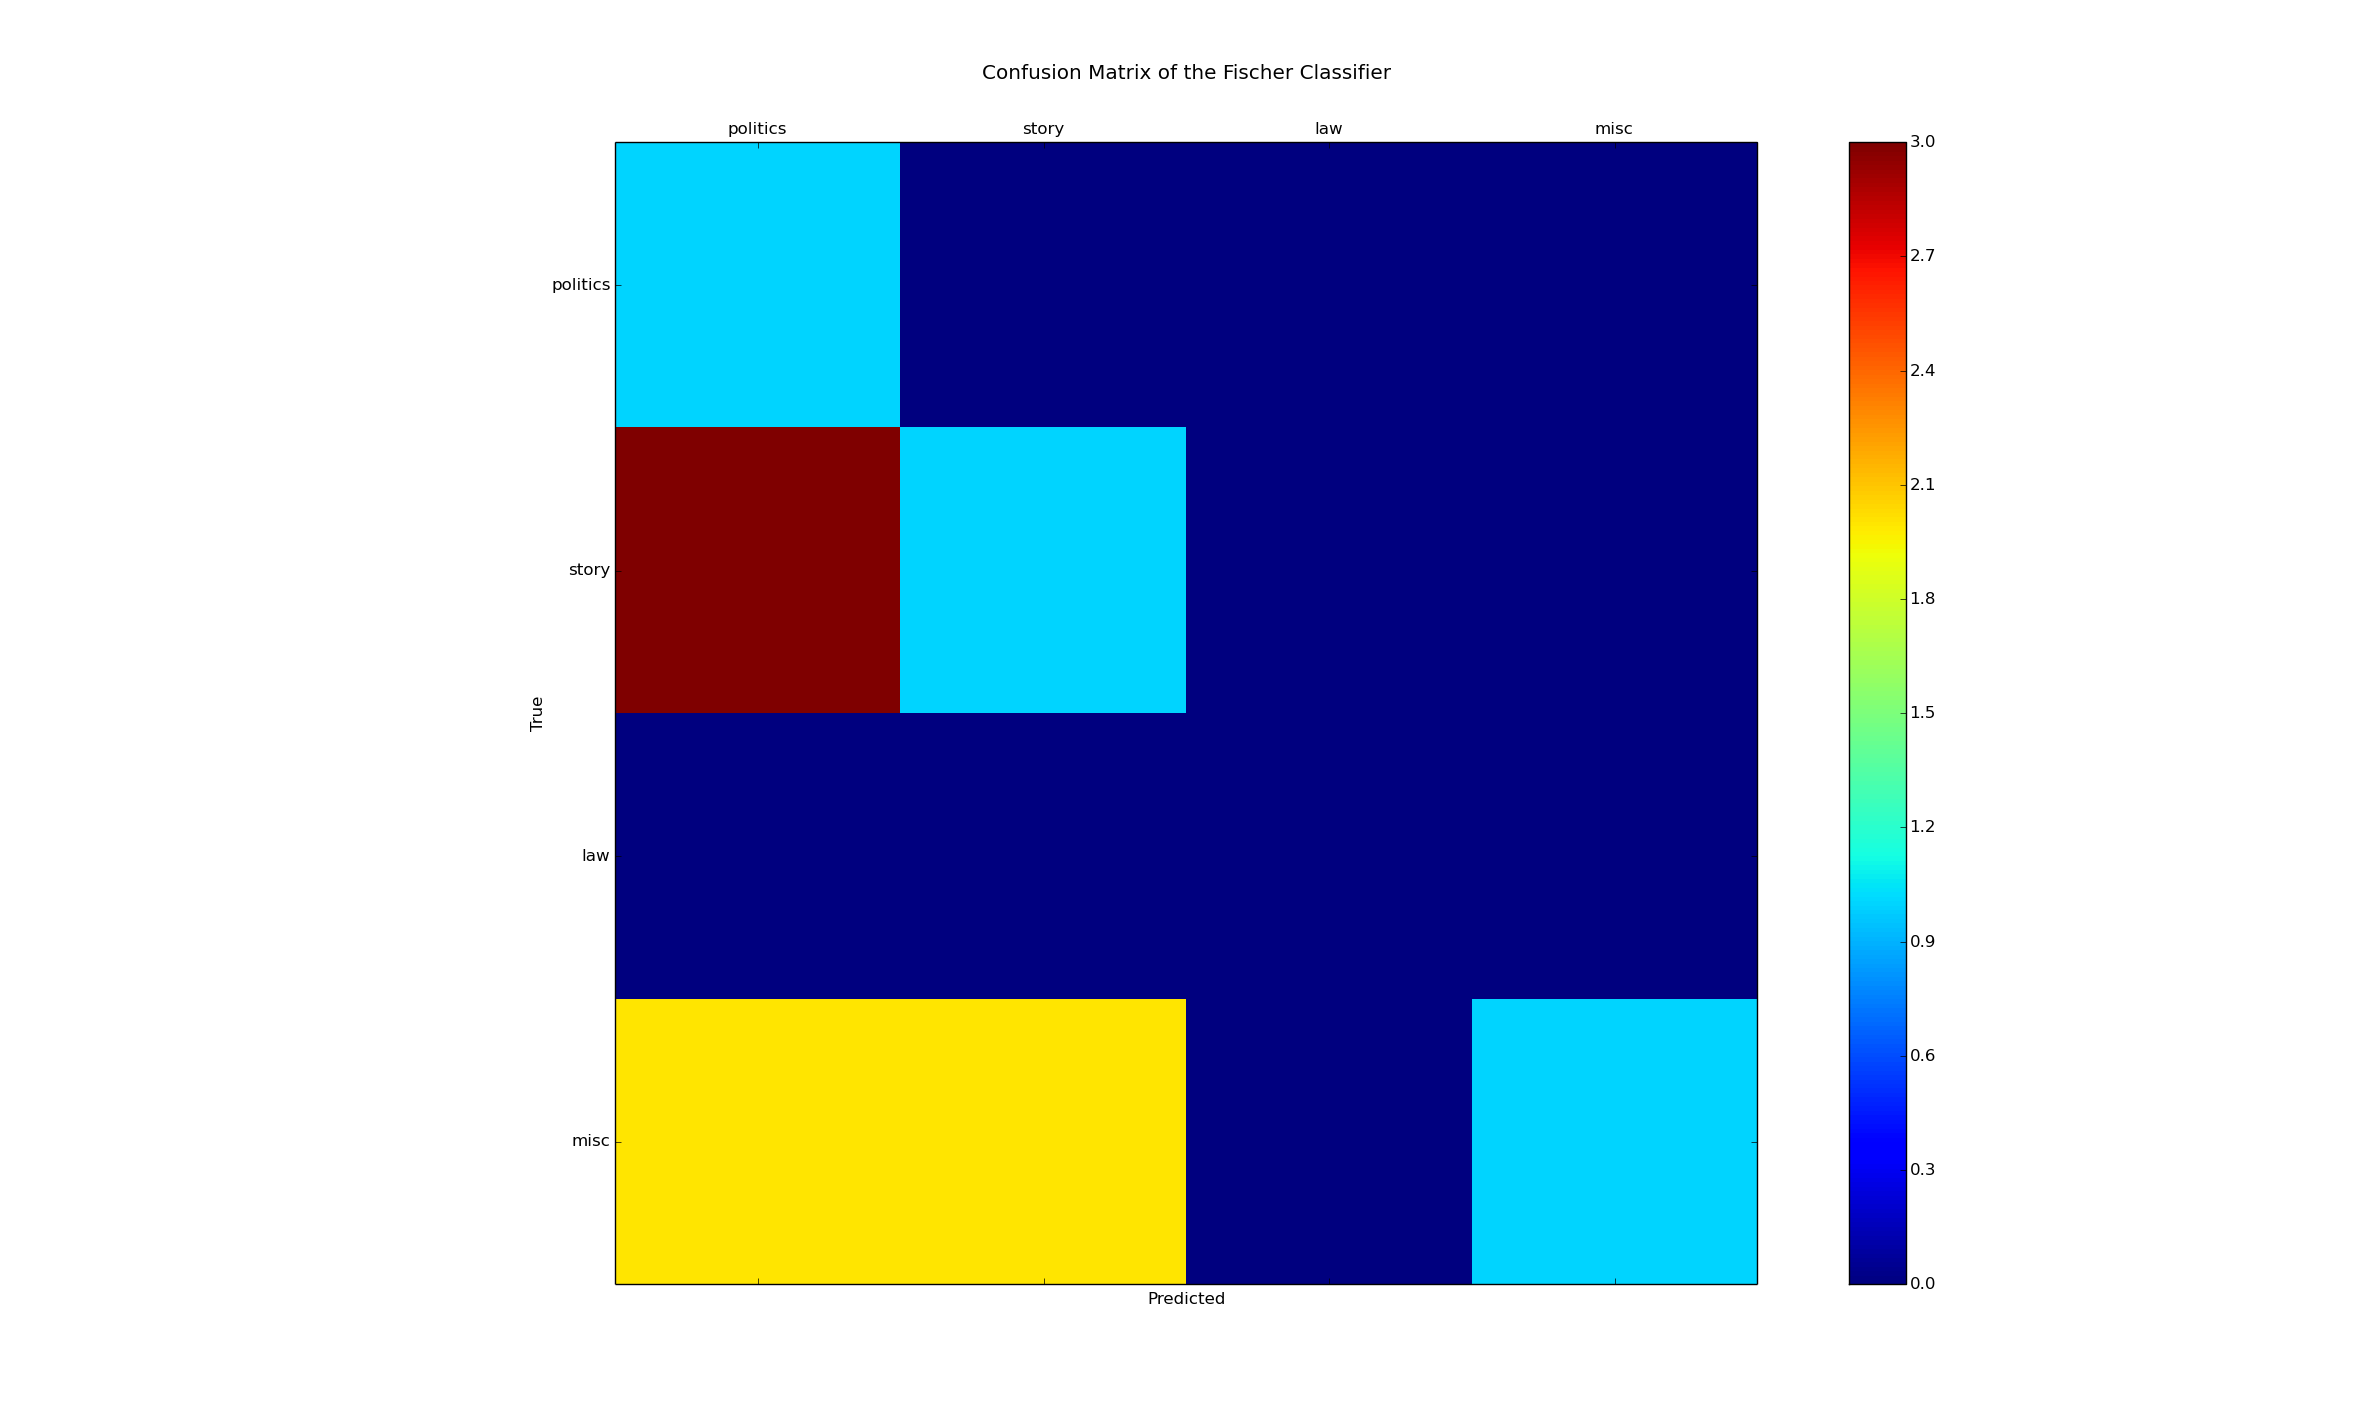
\includegraphics[width=\textwidth]{confusionMatrix2.png}}
\end{figure}

The sum of true positives and false positives are equal to zero for some labels (Law), thus precision/recall/F1 are ill defined.

\item \textbf{Train and test with 50/50 split (improved feature):} The first 50/50 split utilized the getword function for creating the list of features 
(nonalphanumeric split to break up the words). The changes carried out in this train/test operation included in the getfeature function includes the extraction of title words, count of uppercase words and extraction of word pairs. These changes are included in myFisherModelInTrainingAndTesting and nonInteraciveRead (Listing 2.) through the passing of the ``getEntry'' argument.\\

Table 8. outlines the cprop and the prediction/actual labels. Table 7. outlines the precision/recall/F1 measure, Figure 3. outlines the confusion matrix due to the foregoing operation. And below is the corresponding confusion matrix.

\begin{verbatim}
              p   s  l  m
           p [12  0  0  0]
           s [15  5  0  0]
           l [ 4  2  0  0]
           m [ 6  3  0  0]

            p = Politics, s = Story, l = Law, m = Misc
\end{verbatim}

\begin{figure}[h]
    \caption{Confusion Matrix For 50/50 Split With getfeature Function}
    %\subfigure{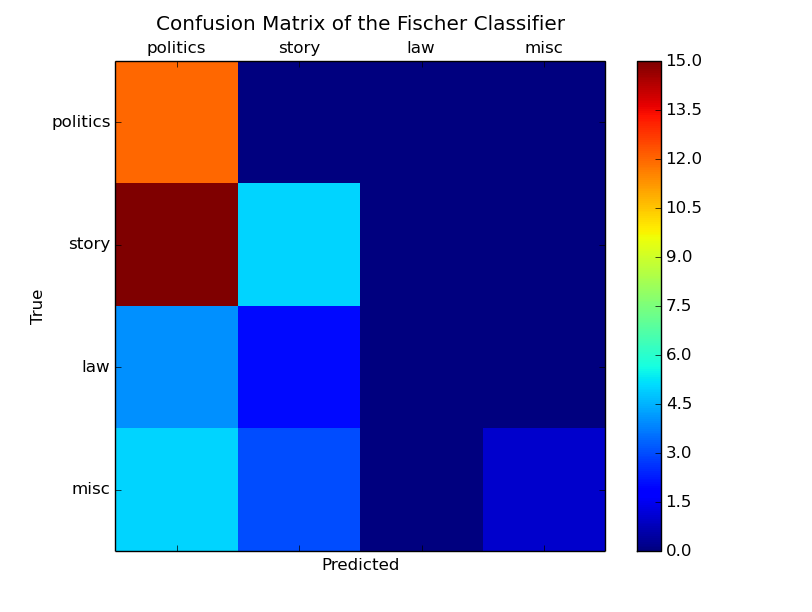
\includegraphics[width=\textwidth,height=\textheight]{confusionMatrix.png}}
    \subfigure{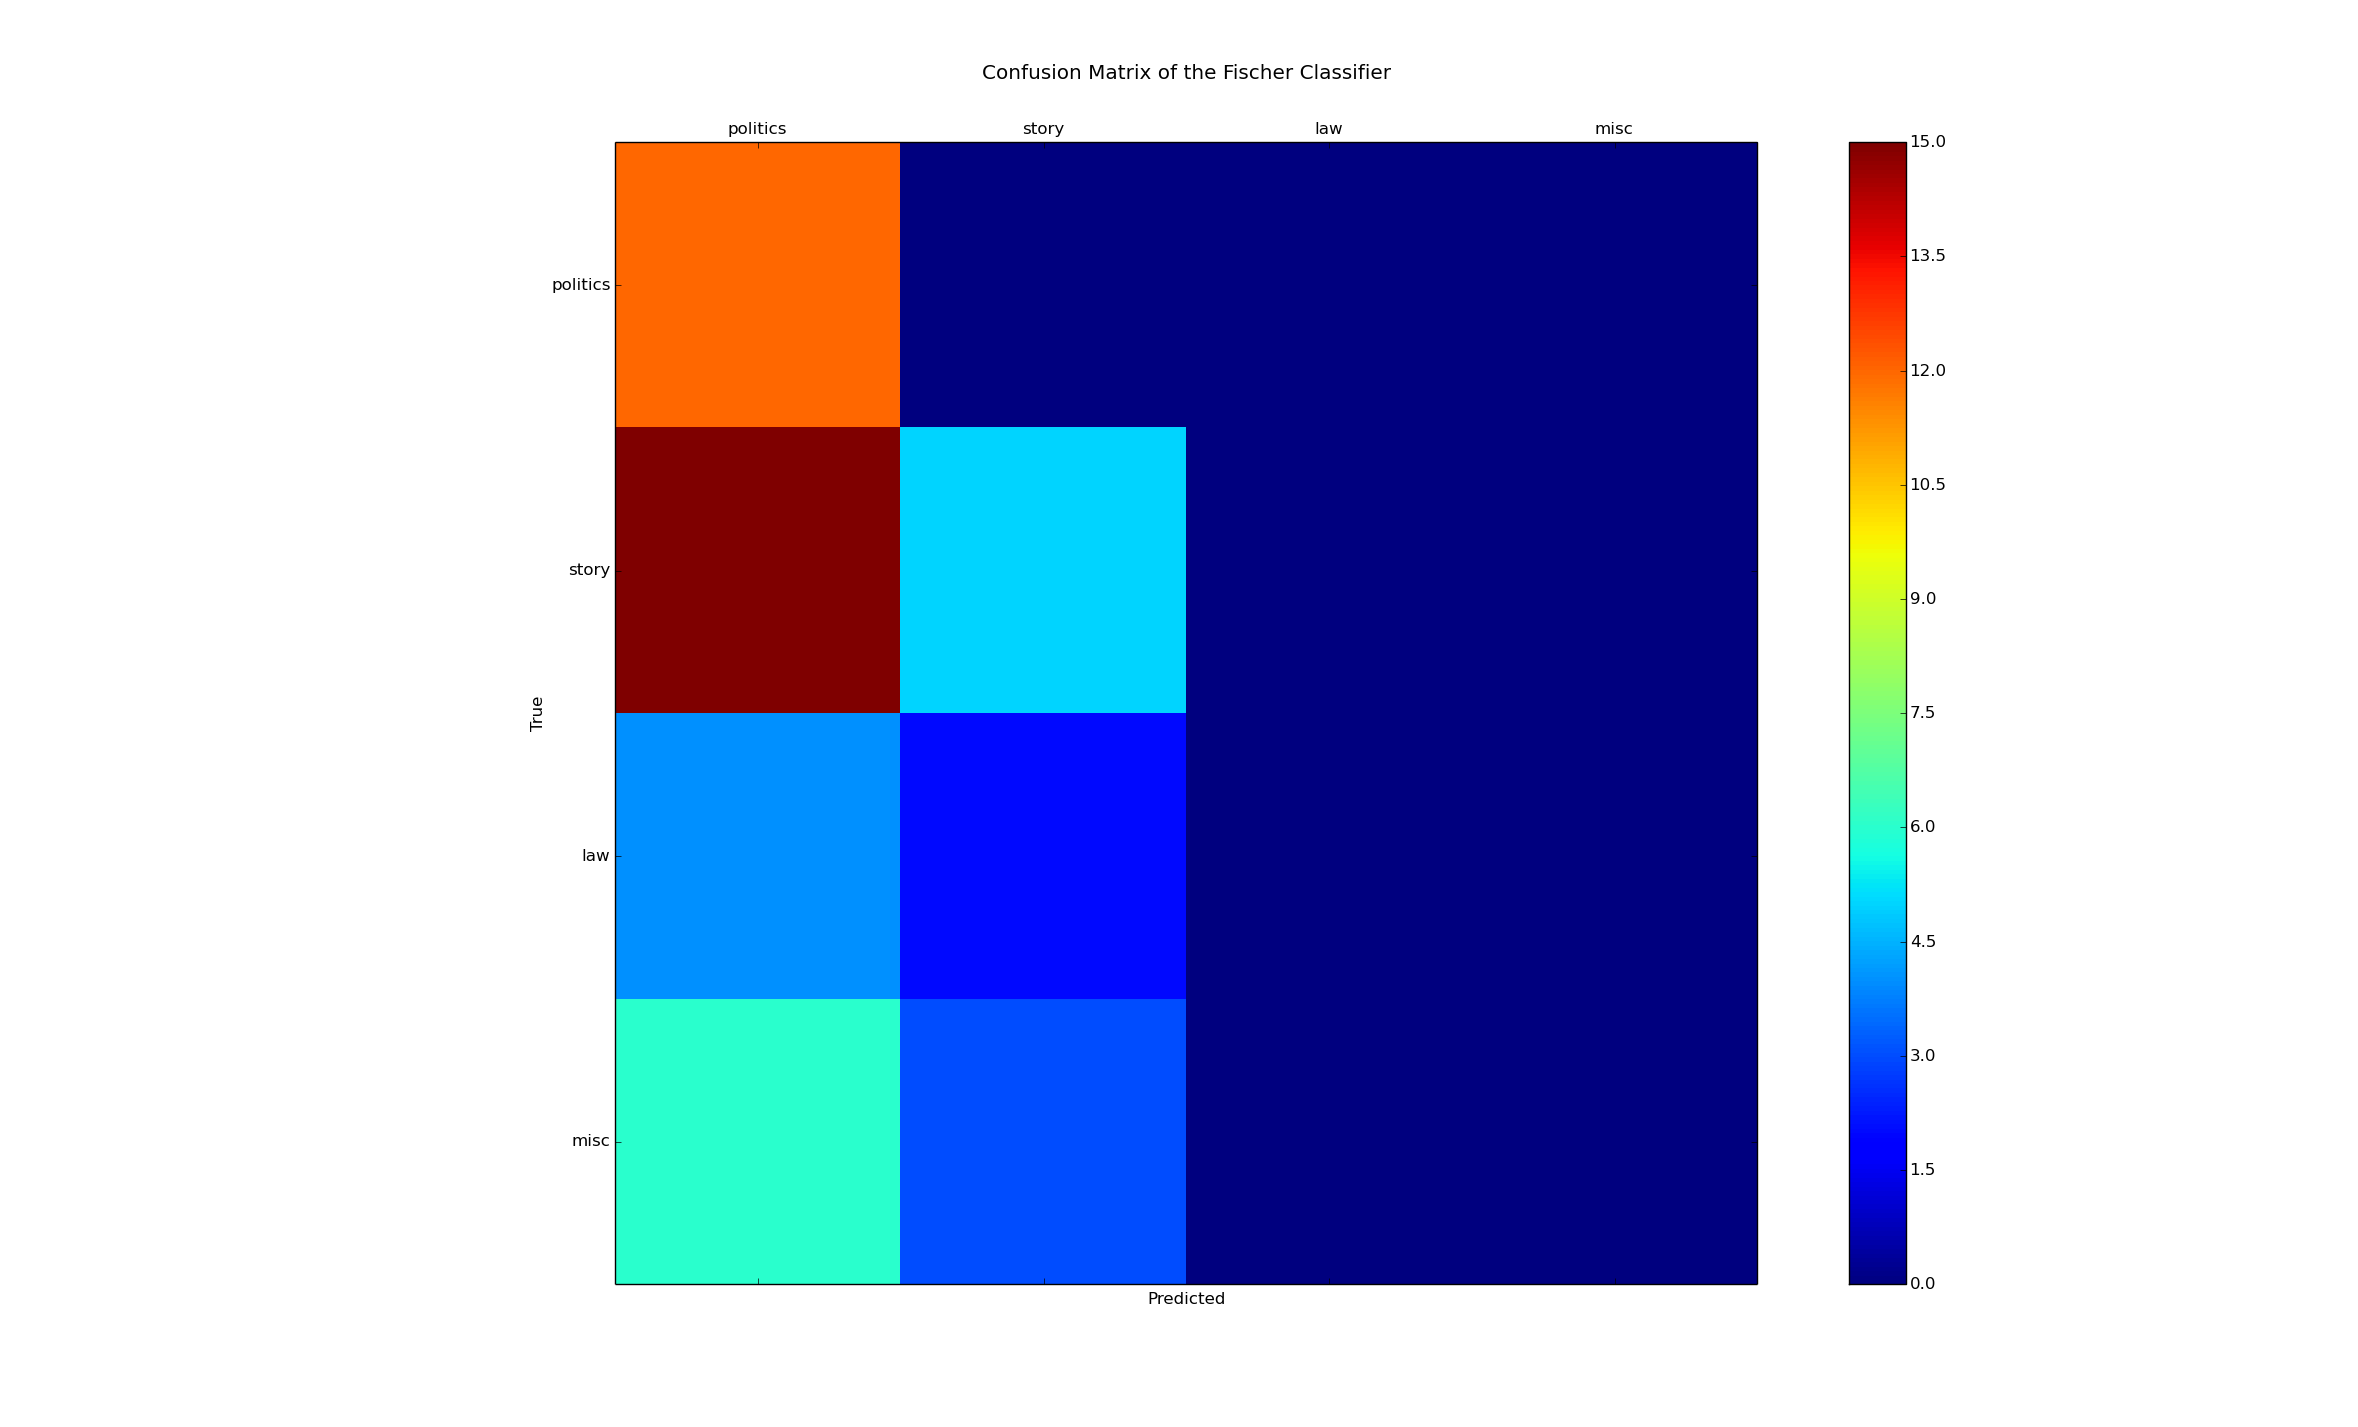
\includegraphics[width=\textwidth]{confusionMatrix3.png}}
\end{figure}

\begin{table}
        \caption{Precision/Recall/F1 Measures For 50/50 Split With getfeature Function} % title of Table
        \centering % used for centering table
        \begin{tabular}{c | c | c | c | c } % centered columns (4 columns)
        \hline\hline %inserts double horizontal lines
        ITEM & Class & Precision & Recall & F1 \\ [0.5ex] % inserts table 
        %heading
        \hline \hline% inserts single horizontal line
        1   &   Politics    &   0.3243  & 1.0000 & 0.4897\\ \hline
        2   &   Story    &   0.5000 & 0.2500 & 0.3333\\ \hline
        3   &   Law    &   0.0000 & 0.0000 & 0.0000 \\ \hline
        4 & Misc & 0.0000 & 0.0000 & 0.0000\\ [1ex] 
        \hline %inserts single line
        \end{tabular}
        \label{table:nonlin} % is used to refer this table in the text
\end{table}

The sum of true positives and false positives are equal to zero for some labels (Law and Misc), thus the measures are ill defined.

\begin{table}
    \caption{Fisher Method Test Result For getfeature Function} % title of Table
    \centering % used for centering table\begin{tabular}{m{5cm} c}
    \begin{tabular}{c | c | c | c | c } % centered columns (4 columns)
    \hline\hline %inserts double horizontal lines
    
    ITEM & ENTRY-TITLE & CPROB & PRED-LABEL & ACTUAL-LABEL \\ [0.5ex] % inserts table 
    %heading
    \hline \hline% inserts single horizontal line

    1   &   Mr. Sulu Phasers Tim Hardaway    &  0.2500 &  story &  misc\\ \hline
    2   &   Too close for comfort       &   0.3693 &  politics &  story\\ \hline
    3   &   Middle School?         &    0.2500 &  politics &  story\\ \hline
    4   &   No kids for gays    &   0.3147 &  politics &  story\\ \hline
    5   &   HDTV       &    0.3693 &  story &  misc\\ \hline
    6   &   Change sometimes isn't so fast         &    0.2500 &  story &  law\\ \hline
    7   &   More idiocy    &    0.2500 &  politics &  politics\\ \hline
    8   &   Yawn, Hillary's In       &  0.2838 &  politics &  politics\\ \hline
    9   &   Scumbags in action         &    0.2500 &  politics &  law\\ \hline
    10   &  The battle of the exploding pigs    &   0.3693 &  politics &  misc\\ \hline

    11   &   Racial Row on UK show            & 0.3693 &  politics &  story\\ \hline
    12   &   No spanking    &   0.3147 &  politics &  story\\ \hline
    13   &   Provoking Sadr      &  0.6018 &  politics &  politics\\ \hline
    14   &   Jenna writes a book            &   0.2500 &  story &  misc\\ \hline
    15   &   Only in Washington    &    0.5058 &  politics &  politics\\ \hline
    16   &   Oooops      &  0.2500 &  politics &  story\\ \hline
    17   &   Another 9/11 tragedy            &  0.3693 &  story &  story\\ \hline
    18   &   Time to serve    & 0.2500 &  politics &  misc\\ \hline
    19   &   About going to Walter Reed      &  0.3693 &  story &  story\\ \hline

    20   &   Voir Dire from hell            &  0.8965  &  politics & law\\ \hline 
    21   &   Simple point    &  0.3693  &  misc & misc\\ \hline
    22   &   Fading away      &  0.8227  &  politics & politics\\ \hline
    23   &   We're playing you            &  0.8333  &  politics & story\\ \hline
    24   &   Libby on trial    &  0.3147  &  politics & law\\ \hline
    25   &   The Car Wreck of American TV      &  0.3693  &  politics & misc\\ \hline
    26   &   No more actors            &  0.2500  &  story & story\\ \hline
    27   &   Good luck, Jane    &  0.2689  &  politics & misc\\ \hline
    28   &   More dead in Iraq      &  0.6132  &  politics & law\\ \hline
    29   &   The good old days my ass            &  0.1575  &  politics & politics\\ \hline

    30   &   A simple question    &  0.8965 &  politics &  law\\ \hline
    31   &   What bubble?      &     0.3693 &  politics &  misc\\ \hline
    32   &   Idiocy in action            &   0.8227 &  politics &  politics\\ \hline
    33   &   Yeah, attacking the Mahdi Army will happen    &     0.8333 &  politics &  story\\ \hline
    34   &   What can I do?      &   0.3147 &  politics &  law\\ \hline
    35   &   Marine murdered for insurance?            &     0.3693 &  politics &  misc\\ \hline
    36   &   Hey, it just happened    &  0.2500 &  story &  story\\ \hline
    37   &   Why the fuck is he making military policy      &    0.2689 &  politics &  misc\\ \hline
    38   &   You have to be kidding            &     0.6132 &  politics &  law\\ \hline
    39   &   Bush will lose the country    &     0.1658 &  politics &  politics\\ \hline

    40   &   Pointless      &  0.2500  &  politics &  story\\ \hline
    41   &   Better to  drop FAE's instead            &  0.2500  &  politics &  story\\ \hline
    42   &   How stupid can you be    &  0.2500  &  story &  story\\ \hline
    43   &   Madness in action      &  0.3147  &  politics &  politics\\ \hline
    44   &   They don't want us            &  0.2500  &  politics &  politics\\ \hline
    45   &   Sucker    &  0.2500  &  politics &  story\\ \hline
    46   &   Silicone    &  0.3693  &  politics &  misc\\ \hline

    47  &  Idiocy in action        &  0.2012  &  politics & story\\ [1ex] 
    \hline %inserts single line
    \end{tabular}
    \label{table:nonlin} % is used to refer this table in the text
\end{table}

\item \textbf{Comparison; which is better getword or getfeature?} Given that some labels have 0 value, only the labels which are present in both models were compared:

\begin{verbatim}

        <Precision (getword), Precision (getfeature)>
        <Politics: 0.3333, Politics: 0.3243>
        <Story: 0.5000, Story: 0.5000>

        <Recall (getword), Recall (getfeature)>
        <Politics: 1.0000, Politics: 1.0000>
        <Story: 0.2500, Story: 0.2500>

        <F1 (getword), F1 (getfeature)>
        <Politics: 0.5000, Politics: 0.4800>
        <Story: 0.3333, Story: 0.5000>

\end{verbatim}

Given that the measures marginally differ, this dataset does not favor any model. However, getfeature is a more sensible way of document classification since is considers more features, as opposed to the monolithic view of getwords.

\end{enumerate}

\end{homeworkProblem}



\begin{verbatim}











\end{verbatim}

\bibliographystyle{plain}
\bibliography{A10bibFile}

%----------------------------------------------------------------------------------------

\end{document}